% Defining a few useful conventions
\newcommand{\fwname}{\texttt{\_fw\_name}}
\newcommand{\surrogateModel}{\texttt{surrogate\_model}}
\newcommand{\surrogateFunction}{\texttt{surrogate\_function}}
\newcommand{\pZero}{\texttt{p0}}
\newcommand{\rhoZero}{\texttt{rho0}}
\newcommand{\pOneByPzero}{\texttt{p1Byp0}}
\newcommand{\diameter}{\texttt{D}}
\newcommand{\id}{\texttt{\_id}}
\newcommand{\cls}{\texttt{\_cls}}
\newcommand{\inputs}{\texttt{inputs}}
\newcommand{\outputs}{\texttt{outputs}}
\newcommand{\fitData}{\texttt{fitData}}
\newcommand{\Min}{\texttt{min}}
\newcommand{\Max}{\texttt{max}}
\newcommand{\argPos}{\texttt{argPos}}
\newcommand{\params}{\texttt{parameters}}
\newcommand{\paramOne}{\texttt{param1}}
\newcommand{\paramTwo}{\texttt{param2}}
\newcommand{\flowRate}{\texttt{flowRate}}
\newcommand{\libraryName}{\texttt{libraryName}}
\newcommand{\functionName}{\texttt{libraryName}}
\newcommand{\Ccode}{\texttt{Ccode}}
\newcommand{\exactTask}{\texttt{exactTask}}
\newcommand{\inheritedInputs}{\texttt{inherited\_inputs}}
\newcommand{\initializationStrategy}{\texttt{initializationStrategy}}
\newcommand{\outofBoundsStrategy}{\texttt{outOfBoundsStrategy}}
\newcommand{\ParameterfittingStrategy}{\texttt{ParameterFittingStrategy}}
\newcommand{\improveErrorStrategy}{\texttt{improveErrorStrategy}}
\newcommand{\initialPoints}{\texttt{initialPoints}}
\newcommand{\nSamples}{\texttt{nSamples}}
\newcommand{\nNewPoints}{\texttt{nNewPoints}}
\newcommand{\maxerror}{\texttt{maxerror}}
\newcommand{\maxIterations}{\texttt{maxIterations}}
\newcommand{\testDataPercentage}{\texttt{testDataPercentage}}
\newcommand{\outsidePoint}{\texttt{outsidePoint}}
\newcommand{\surrFunction}{\texttt{surrogateFunction}}
\newcommand{\tst}{\texttt{test}}
\newcommand{\lcl}{\texttt{local}}
\newcommand{\fireworks}{\texttt{fireworks}}
\newcommand{\sysIndex}{\texttt{system.indexes}}
\newcommand{\catOne}{\texttt{cat\_1.}}
% --------------------------------------------------------------- %
%%                                                               %%
%%%                                                             %%%
%%                                                               %%
% --------------------------------------------------------------- %
\section{Database concept}
    \label{sec:database}
%
A database can be defined as an organized collection of data which
enables us to handle large quantities of information by inputting, storing,
retrieving and managing them.  A relational database is defined as a database in
which the data is organized based on the relational model of data.
\cite{codd_and_edgar_1970} The purpose of this model is to provide a declarative
method for data and query specification.  Relational databases mostly use
structured query language ({\SQL}) which can also be used as a term to describe
a relational database.

Non-relational databases, dubbed as {\NoSQL} (Not Only {\SQL}), provide a
mechanism for storage and retrieval of data which is modeled in a way different
than in a relational database.  \cite{nasholm_2012} {\NoSQL} databases are of
interest in {\MoDeNa} project since they allow database schemas which adapt to
the users needs in a seemless manner. {\MongoDB} is a auch a {\NoSQL} document
store database written in {\CPP} and developed in an open-source project by the
company 10gen Inc.  The motivation behind its development is to close the gap
between the fast and highly scalable key-value-stores and feature-rich
traditional relational database management systems.  \cite{shermin_2013}

Some fundamental features of {\MongoDB} are listed below to provide a more
concrete insight and detailed information about the terminology and concepts:
\begin{itemize}
\item Document database: A record in {\MongoDB} is a document which is a data
  structure composed of field and value, or key and value pairs.  The values of
  fields can also include other documents, arrays, and arrays of documents.
  {\MongoDB} documents are in {\BSON} ('Binary {\JSON}') data format.
  Essentially, it is a binary form for representing objects or documents.  Using
  document is advantageous since the documents correspond to native data types
  in many programming languages, embedded documents (subdocuments) and arrays
  reduce need for expensive joins, and dynamic schema supports fluent
  polymorphis.  \cite{MongoDBManual} In the documents, the value of a field can
  be any of the {\BSON} data types, including other documents, arrays, and
  arrays of documents.  {\MongoDB} stores all documents in collections.  A
  collection is a group of related documents that have a set of shared common
  indexes.  Collections are analogous to a table in relational databases.
\item High performance: {\MongoDB} provides high performance data persistence.
  In particular, support for embedded data models reduces I/O activity on
  database system, and indexes support faster queries and can include keys from
  embedded documents and arrays. \cite{MongoDBManual}
\item High availability: To provide high availability, {\MongoDB}'s replication
  facility, called replica sets, provide automatic failover and data redundancy.
  A replica set is a group of {\MongoDB} servers that maintain the same data
  set, providing redundancy and increasing data availability.
  \cite{MongoDBManual}
\item Automatic scaling: {\MongoDB} provides horizontal scalability as part of
  its core functionality.  Automatic sharding distributes data across a cluster
  of machines.  Replica sets can provide eventually-consistent reads for
  low-latency high throughput deployment. \cite{MongoDBManual}
\end{itemize}
%
\begin{table}
  \centering
  \caption{Terminology and concepts in {\SQL} and {\MongoDB} \cite{MongoDBManual}.}
  \begin{tabular}{l l}
    \hline
    {\SQL} & {\MongoDB} \\ \hline \hline
    Database & Database \\
    Table & Collection \\
    Row & Document or {\BSON} Document \\
    Column & Field \\
    Index & Index \\
    Table joins & Embedded documents and linking \\
    Primary key (specify any unique column or column combinations as primary key) & Primary key (the primary key is automatically set to the {\id} field in {\MongoDB}) \\
    Aggregation (e.g. by group) & Aggregation pipeline \\
    \hline
  \end{tabular}
  \label{tab:terminology}
\end{table}
%
To provide insight in {\MongoDB} in a comparative manner with more widely used
relational database ({\SQL}) approach, terminology and concepts of these two are
summarized and shown in Table \ref{tab:terminology}.

{\MongoDB} implements the basic functions of data storage, initially defined for
{\SQL}: (create, read, update, delete) {\CRUD}. In {\MongoDB}, these are
represented as query which corresponds to read operations while data
modification stands for create, update and delete operations.  In {\MongoDB},
read operation is a query which targets a specific collection of documents.
Queries specify criteria, or conditions, that identify the documents that
{\MongoDB} returns to the clients.  A query may include a projection that
specifies the fields from the matching documents to return.

{\MongoDB} queries exhibit the following behavior:
\begin{itemize}
\item All queries in {\MongoDB} address a single collection.
\item Queries can be modified to impose limits, skips, and sort orders.
\item The order of documents returned by a query is not defined unless a
  \texttt{sort()} method is used.
\item Operations that modify existing documents use the same query syntax as
  queries to select documents to update.
\item In aggregation pipeline, the \$ match pipeline stage provides access to
  {\MongoDB} queries.
\end{itemize}

\begin{figure}
  \psset{unit=0.2}
  \centering
  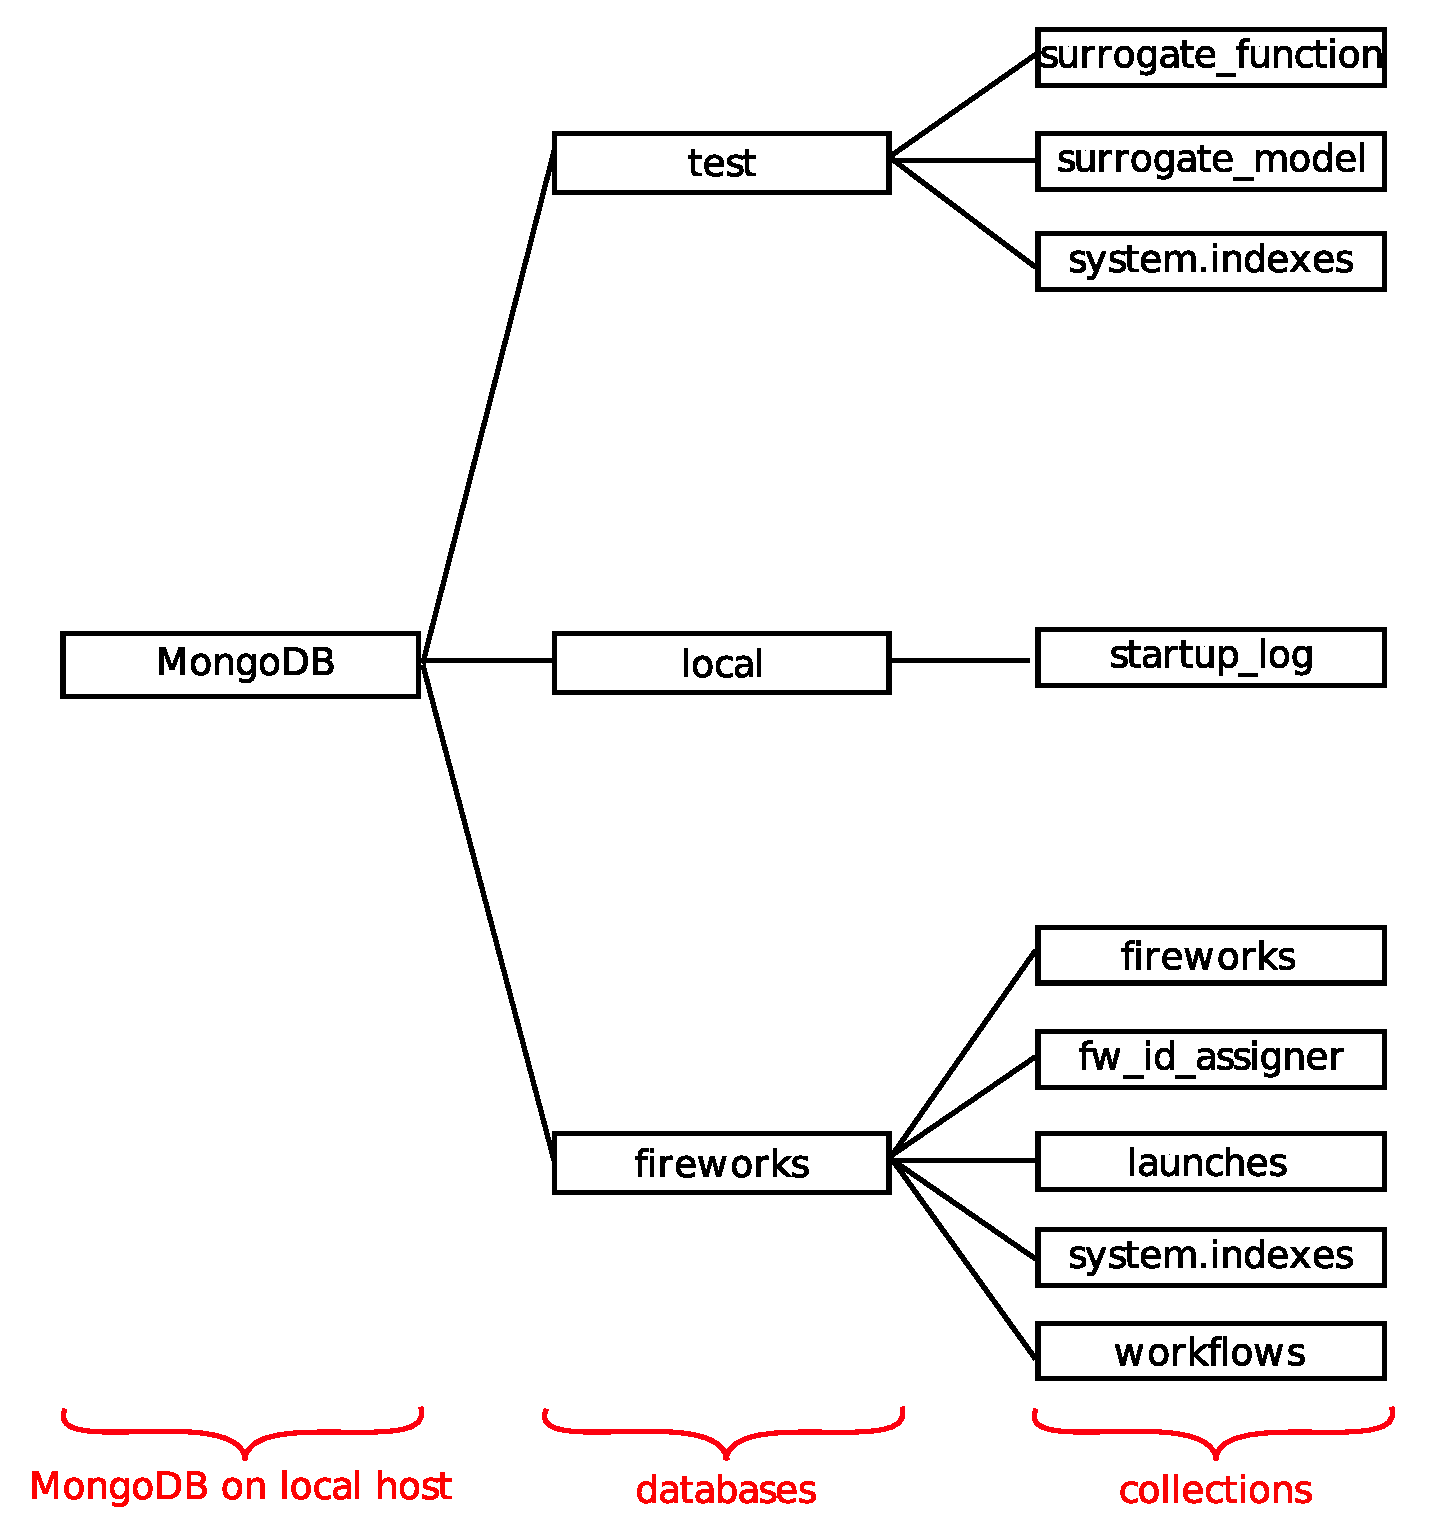
\includegraphics[width=0.75\textwidth,keepaspectratio=true]{./Content/Figures/mongodb_on_local_host.eps}
  \caption{Illustration of database organization in {\MongoDB} on a local host.}
  \label{fig:MongoDBlocal}
\end{figure}
%
The {\MoDeNa} project uses {\MongoDB} for data storage.  As shown in Figure
\ref{fig:DataFlow}, the database has a crucial role as it resides in the core of
the flow of information.  In {\MongoDB}, when there is data insertion, default
database named as {\tst} is automatically populated unless specified otherwise.
The test database in {\MoDeNa} project contains information regarding
\emph{work-flow}, \emph{work-flow state}, \emph{models}, \emph{experiments},
\emph{metadata}, \emph{simulation context}.  Moreover, the software,
{\Fireworks} used in the project also employs {\MongoDB} for \emph{work-flow}
(FireTasks) storage in a database called as {\fireworks}.  In addition to {\tst}
and {\fireworks} databases, there is another database ({\lcl}) that is
automatically created by {\MongoDB} for the purpose of saving log information.
Figure \ref{fig:MongoDBlocal} shows an illustration of the {\MongoDB} databases
and corresponding collections.
%
As can be seen in Figure \ref{fig:MongoDBlocal}, there are three {\MongoDB}
databases ({\tst}, {\lcl}, {\fireworks}) on local host and their corresponding
collections are also shown.  In {\MongoDB}, the system generates the name by
concatenating the index key field and value with an underscore, e.g. {\catOne},
if the user does not specify an index name \cite{MongoDBManual}, and they are
stored in a collection named as {\sysIndex} which can be observed in the figure
both for the {\tst} and {\fireworks} databases.  Each collection has at least one
document which are not shown in the figure.
%
Since the local database is generated by {\MongoDB} and {\fireworks} database structure
is defined by the software itself, the main focus will be the test database
which is developed within the scope of the {\MoDeNa} project.  For twoTank
example in the project, data is stored in test database as well which has 3
collections: {\surrogateFunction}, {\surrogateModel} and system.indexes.  Each
collection stores documents which consist of key and value pairs.
%
\begin{figure}
  \psset{unit=0.2}
  \centering
  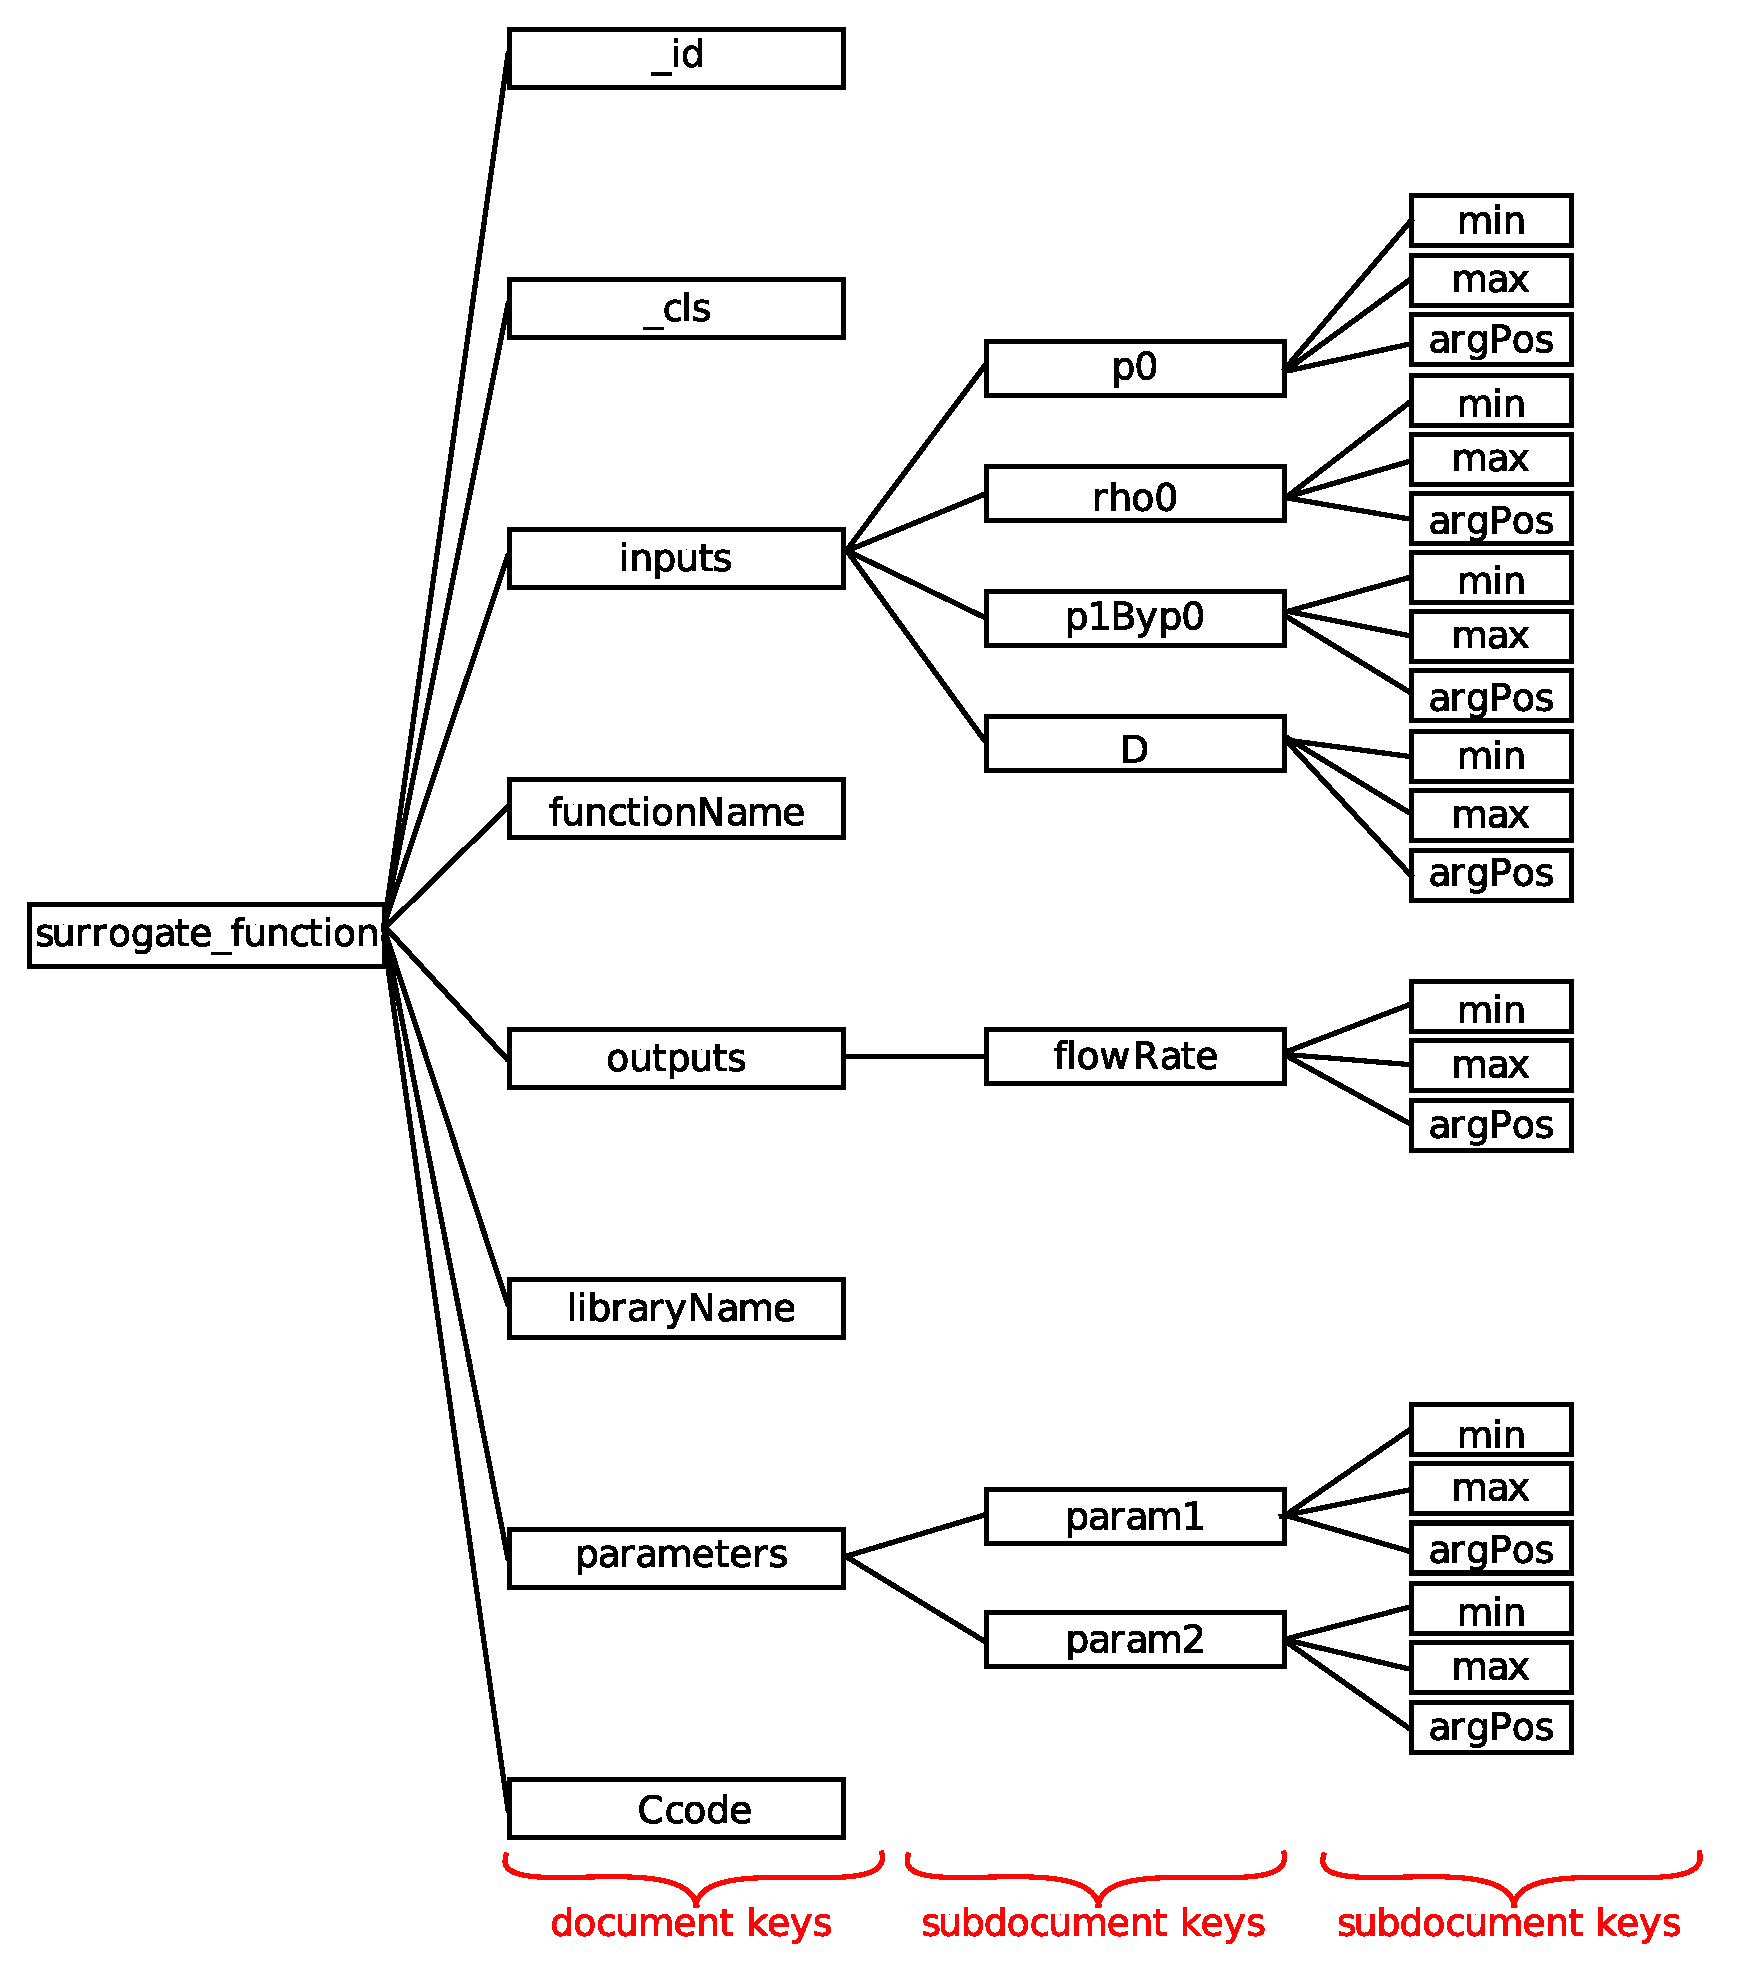
\includegraphics[width=0.75\textwidth,keepaspectratio=true]{./Content/Figures/surrogate_function.eps}
  \caption{Data schema of {\surrogateFunction} collection.}
  \label{fig:surrogatefunction}
\end{figure}
%
The collection, {\surrogateFunction} contains one single document with the keys:
id of the function \id; class of the function, {\cls}; the global bounds for the
function, {\inputs} which are {\pZero}, {\rhoZero}, {\pOneByPzero} and
{\diameter}, {\outputs} which is {\flowRate} and {\params} which are {\paramOne}
and {\paramTwo} with global minimum value {\Min}, global maximum value {\Max}
and argument position {\argPos}; name of the function {\functionName}; compiled
model in the library {\libraryName}; {\Clang}-code of the function for model
execution and parameter estimation {\Ccode}.  All the mentioned keys and their
value, and the hierarchy between them in terms of subdocuments constitute the
database schema.  The database schema is specified with corresponding keys and
values in the initialization script except {\libraryName} whose value is
compiled in surrogatemodel script.  To illustrate the data structure, data
schema for {\surrogateFunction} collection is drawn with keys and it is shown in
Figure \ref{fig:surrogatefunction}.
%
As can be seen in Figure \ref{fig:surrogatefunction}, {\surrogateFunction}
collection has one document which has 8 keys ({\id}, {\cls}, {\inputs},
{\functionName}, {\outputs}, {\libraryName}, {\params}, {\Ccode}).  Three of the
keys store documents as values e.g. subdocuments ({\pZero}, {\rhoZero},
{\pOneByPzero}, {\diameter}, {\flowRate}, {\paramOne}, {\paramTwo}), and
subdocuments also store documents ({\Min}, {\Max} and {\argPos}).  Thus, there
are three levels of hierarchy in the data structure.
%
\begin{figure}
  \psset{unit=0.2}
  \centering
  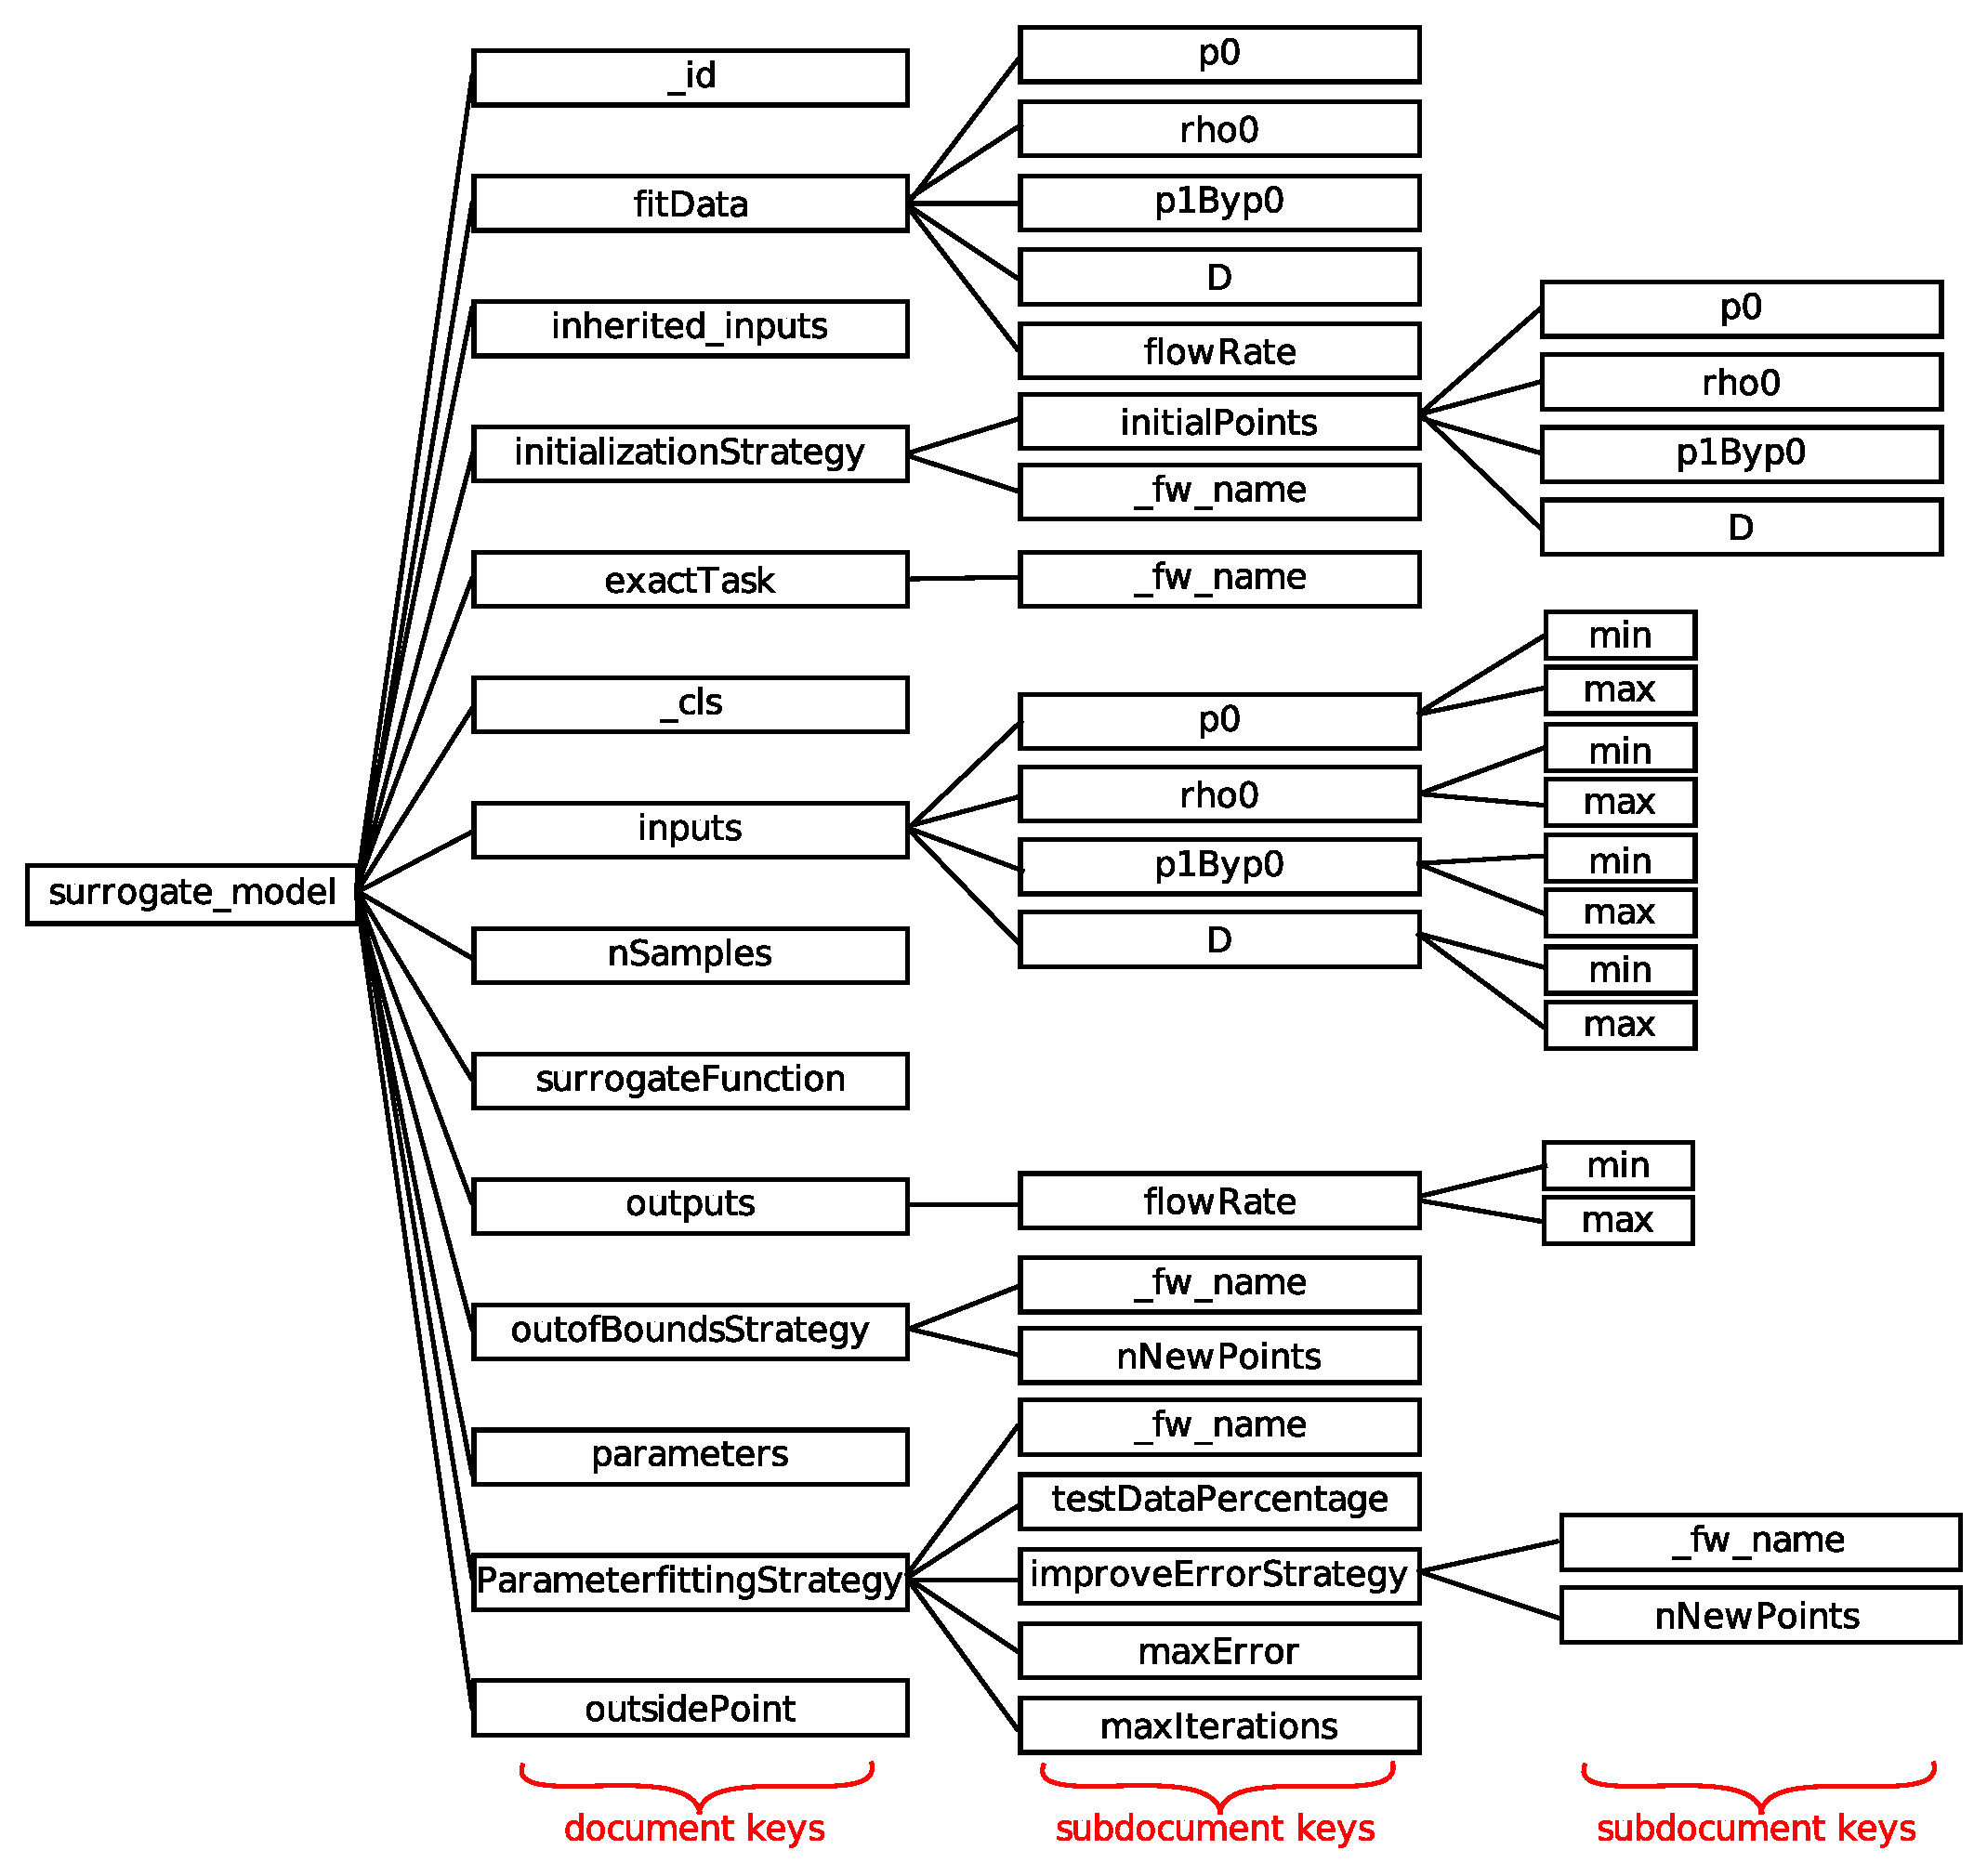
\includegraphics[width=0.75\textwidth,keepaspectratio=true]{./Content/Figures/surrogate_model.eps}
  \caption{Data schema of {\surrogateModel} collection.}
  \label{fig:surrogatemodel}
\end{figure}
%
The collection, {\surrogateModel} contains also one single document with the
keys: class of the model, {\cls}; id of the model {\id}; Firework spec
{\exactTask} which has a name of {\fwname}; fitting data {\fitData} which are
{\pZero}, {\rhoZero}, {\pOneByPzero} and {\diameter}; inherited inputs
{\inheritedInputs}; initialization strategy {\initializationStrategy} which has
{\initialPoints} of {\pZero}, {\rhoZero}, {\pOneByPzero} and {\diameter}, and a
name of {\fwname}; the global bounds for the function, {\inputs} which are
{\pZero}, {\rhoZero}, {\pOneByPzero} and {\diameter} with global minimum value
{\Min}, global maximum value {\Max}; number of sample points {\nSamples};
determination of points outside of the bounds {\outofBoundsStrategy} and
corresponding number of points {\nNewPoints} and a name of {\fwname}; output of
the calculation {\outputs} which is {\flowRate} with global minimum value
{\Min}, global maximum value {\Max}; parameter fitting strategy
{\ParameterfittingStrategy} with maximum error limit of {\maxerror},
sub-strategy for improvement {\improveErrorStrategy} and corresponding number of
points {\nNewPoints} and a name of {\fwname}, maximum number of iterations
{\maxIterations}, name of {\fwname} and {\testDataPercentage}; {\params},
corresponding function of the model {\surrFunction} and calculated numbers
outside of bounds {\outsidePoint}.  To illustrate the data structure, data
schema for {\surrogateModel} collection is drawn with keys and it is shown in
Figure \ref{fig:surrogatemodel}.
%
As can be seen in Figure \ref{fig:surrogatemodel}, {\surrogateModel}
collection has one document which has 14 keys ({\id}, {\fitData},
{\inheritedInputs}, {\initializationStrategy}, {\exactTask}, {\cls},
{\inputs}, {\nSamples}, {\surrFunction}, {\outputs},
{\outofBoundsStrategy}, {\params}, {\ParameterfittingStrategy},
{\outsidePoint}).  As described in Figure \ref{fig:surrogatefunction},
keys store documents e.g. subdocuments.  Thus, there are three levels
of hierarchy in the data structure.
